
\documentclass[a4paper,11pt, ngerman]{scrartcl}
\addtokomafont{disposition}{\rmfamily}
\usepackage[utf8]{inputenc}
\usepackage[german]{babel}
\usepackage[T1]{fontenc}
\usepackage{amsmath}
\usepackage{amsfonts}
\usepackage{amssymb}
\usepackage{amsthm}
\usepackage{graphicx}
\usepackage{rotating}
\usepackage{paralist}
\usepackage{setspace}
\usepackage{pdfpages}
\usepackage{pdflscape}
\usepackage{longtable}
\usepackage{listings}
\usepackage{algorithm}
\usepackage{enumitem}
\usepackage{cancel}
\usepackage{wrapfig}
\usepackage[noend]{algpseudocode}
\usepackage[pdfborder={0 0 0}]{hyperref}
\usepackage{cleveref}
\usepackage{array}
\usepackage{float}
\usepackage{parallel}
\usepackage[left=2.5cm,right=2.5cm,top=3cm,bottom=3cm]{geometry}
\usepackage{scrpage2}
\usepackage{bibgerm}
\usepackage[style=numeric, maxcitenames=2, backend=bibtex]{biblatex}
\usepackage[babel,german=quotes]{csquotes}

\usepackage{relsize}
\usepackage{subcaption}

\setcapindent{1em}

\defbibheading{head}{\chapter{Quellen und verwendete Ressourcen}}

\lstset{
basicstyle=\footnotesize,
frame=single,
language=C++,
captionpos=b,
breaklines=true,
columns=flexible,
tabsize=4
}

\makeatletter
\def\clearwf{\par{\count@\c@WF@wrappedlines\zz}\par}

\def\zz{{%
\ifnum\count@>\@ne
\noindent\mbox{~~}\\%
\advance\count@\m@ne
\expandafter\zz
\else
\ifhmode\unskip\unpenalty\fi
\fi}}

\makeatother

\newtheorem{definition}{Definition}
\newtheorem{lemma}[definition]{Lemma}
\newtheorem{example}[definition]{Beispiel}
\crefname{chapter}{Kapitel}{Kapitel}
\crefname{section}{Abschnitt}{Abschnitte}
\crefname{lemma}{Lemma}{Lemmata}
\crefname{definition}{Definition}{Definitionen}
\crefname{example}{Beispiel}{Beispiele}
\crefname{figure}{Abbildung}{Abbildungen}
\crefname{line}{Zeile}{Zeilen}
\crefname{algorithm}{Algorithmus}{Algorithmen}
\crefname{lstlisting}{Codeausschnitt}{Codeausschnitte}
\crefname{listing}{Codeausschnitt}{Codeausschnitte}
\floatname{algorithm}{Algorithmus}


\renewcommand{\i}{\ensuremath{\mathrm{i}}}
\newcommand{\true}{\ensuremath{\text{true}}}
\newcommand{\false}{\ensuremath{\text{false}}}

\renewcommand{\lstlistingname}{Codeausschnitt}% Listing -> Algorithm
\renewcommand{\lstlistlistingname}{Liste der \lstlistingname e}

\renewcommand*\listalgorithmname{Algorithmenverzeichnis}
\algnewcommand\algorithmicinput{\textbf{Input:}}
\algnewcommand\INPUT{\item[\algorithmicinput]}
\algnewcommand\algorithmicoutput{\textbf{Output:}}
\algnewcommand\OUTPUT{\item[\algorithmicoutput]}
\MakeRobust{\Call}


\usepackage{titling}
\pretitle{\begin{flushleft} \end{flushleft}\vskip 2em
\begin{flushright}\LARGE}
\posttitle{\par\end{flushright}\vskip 0.5em}
\preauthor{\vfill\begin{flushright}\large \lineskip 0.5em}
\postauthor{{}\\\authorAddon\par\end{flushright}}
\predate{\begin{flushright}\large}
\postdate{\par\titlehead\end{flushright}}
\renewcommand*{\postnotedelim}{\addcolon\space}
\DeclareNameAlias{sortname}{last-first}
\DeclareNameAlias{default}{last-first}
\DeclareFieldFormat{postnote}{#1}
\DeclareFieldFormat{pages}{#1}
\renewcommand{\cite}{\parencite}
\renewcommand*{\multinamedelim}{/\space}
\renewcommand*{\finalnamedelim}{/\space}

\pagestyle{scrheadings}
\renewcommand{\titlehead}{Ausarbeitung\\ Hardwarenahe Systemprogrammierung\\
Prof. Dr. Sturm}
\newcommand{\authorAddon}{}
\author{Christian Stahl\\Nico Feld}
%\title{Julia-Mengen quadratischer Funktionen\\{\smaller Approximation und Garantien pixelbasierter Algorithmen}}
\title{Bau eines Wardriving-Moduls}
\date{\today}

\newcommand{\param}[1]{{\smaller Parameter: \lstinline!#1!}}

\begin{document}
\pagenumbering{gobble}
\maketitle
\pagebreak
\pagenumbering{arabic}
\tableofcontents
\pagebreak
%\listoffigures
%\listofalgorithms
%\lstlistoflistings
%\listoftables
\section{Motivation \& Idee}
Diese Arbeit beschäftigt sich mit dem Erstellen eines Wardriving-Moduls. \grqq Wardriving\grqq{} bezeichnet dabei das systematische Erfassen von WLAN-Netzen an verschiedenen Positionen und deren anschließender Auswertung. Anschließend können dann die erfassten WLAN-Netze der Position zugeordnet werden und letztendlich kartographiert werden. Dafür wird ein extra Modul mit Positionsbestimmung (GPS) und WLAN-Komponente benötigt. Als Motivation kann einerseits das Finden von unsicheren Netzwerken und der anschließenden Meldung an den Besitzer oder aber auch einfach die Kartographie von offenen WLAN-Netzen für Touristen o.Ä. Im Rahmen des Moduls \grqq Hardware-nahe Programmierung\grqq{} haben wir sein solches Modul sowohl programmiert als auch zusammengebaut. Dabei haben wir das Modul um die Funktion erweitert Bluetooth-Geräte und ursprünglich auch die Netzabdeckung via GSM-Modul zu erfassen.
\section{Aufbau \& Probleme}
Zur Erfassung der GPS-Daten, der WLANs, der Bluetooth-Ger"ate, sowie der GSM-Abdeckung, haben wir die verschiedenen Module sternf"ormig um einen Teensy 3.6 angeordnet, welcher die zentrale Koordination und Datenspeicherung "ubernimmt. Die verschiedenen Module werden per UART verbunden, die Spannungsversorgung liefert eine Powerbank per USB, teils wird sie "uber den Teensy weitergereicht. Dazu verwenden wir, wie in \cref{abb:compl} zu sehen, rote und schwarze Dr"ahte, um sie von den Leitungen f"ur logische Pegel zu unterscheiden.\\
Bei Start unseres Moduls initialisiert der Teensy die angeschlossenen Module. Anschlie"send wird in einer Schleife stets zun"achst die GPS-Information abgefragt. Um Endlosschleifen zu vermeiden wurden alle Module um eine Abbruchbedingung (kill-count) erweitert, sodass kein Modul den Gesamtablauf blockieren kann. Sollte nach der gegebenen Anzahl Versuche keine verwertbare Information erfasst sein, so bricht die Erfassung des einzelnen Moduls ab. Wird kein GPS-Punkt gefunden, so haben wir die anderen Module nicht abgefragt, sondern eine Wartezeit von 20 Sekunden eingebaut, um zu verhindern, dass die Module hei"s laufen, was bei ersten Implementierungen zu Problemen f"uhrte.

\begin{figure}[H]
	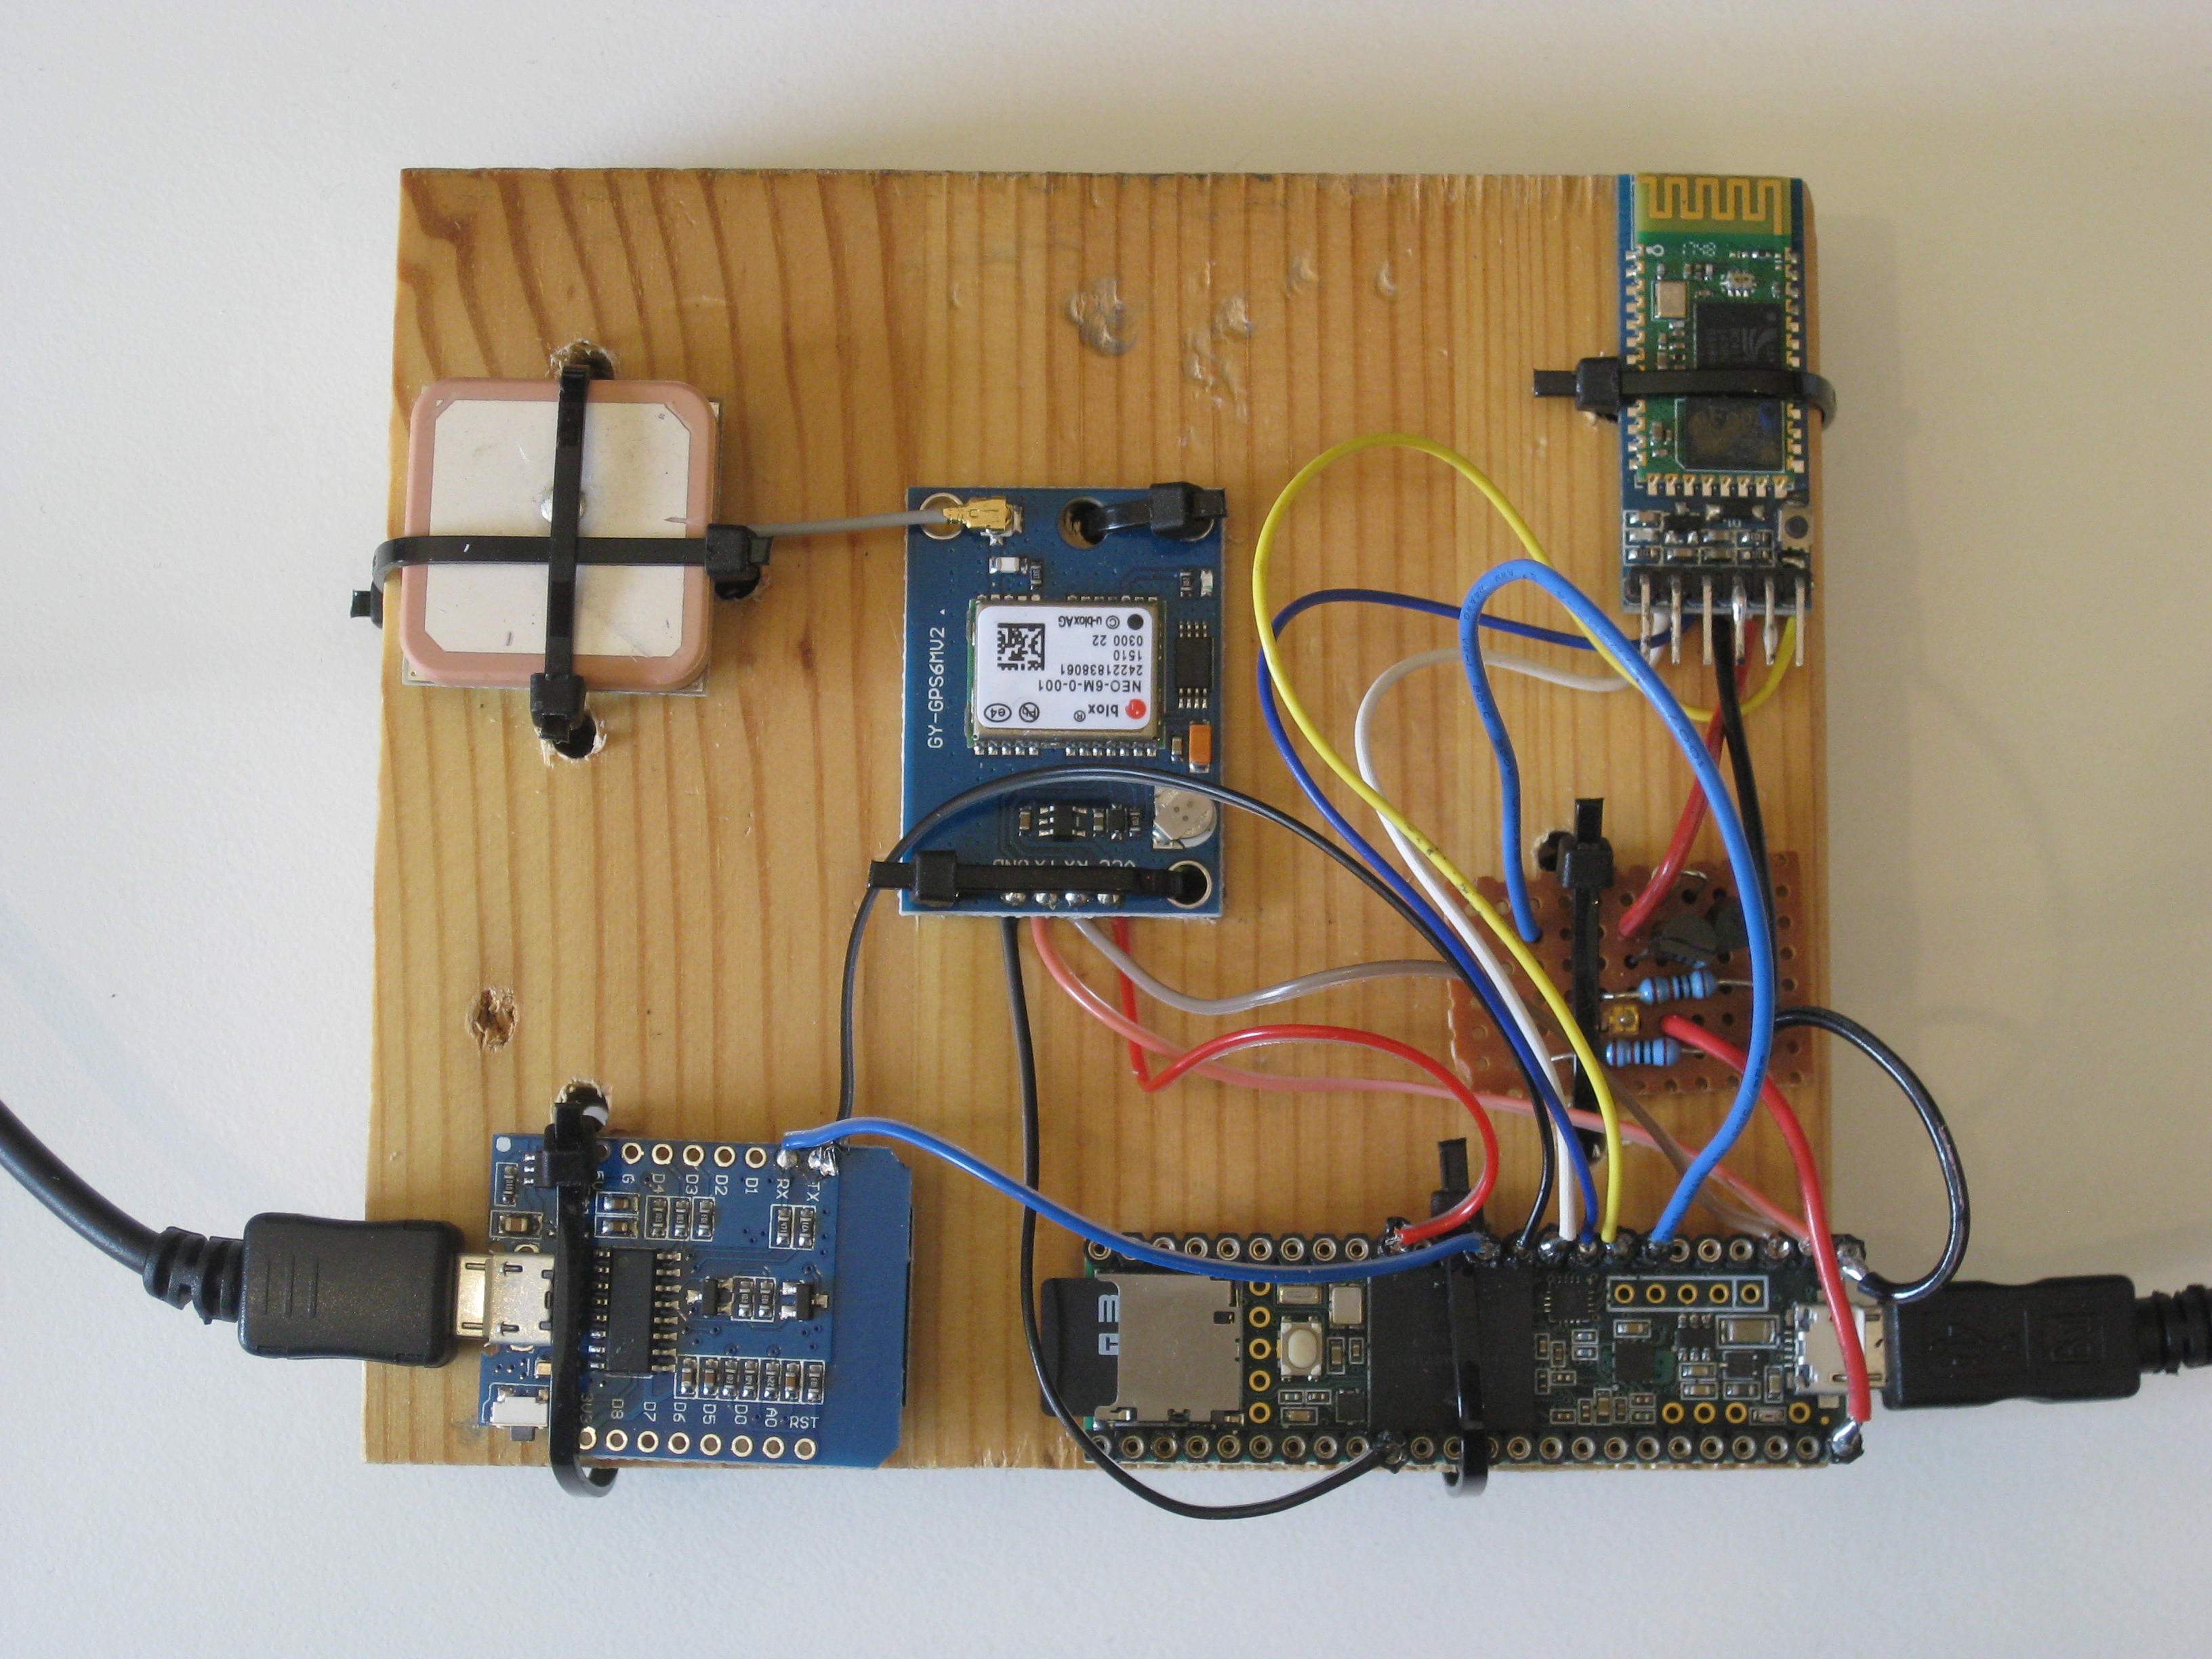
\includegraphics[width=.95\linewidth]{Aufbau.JPG}\caption{Aufbau unseres Wardriving-Moduls}\label{abb:compl}
\end{figure}

\subsection{Teensy 3.6}
Als programmierbares \grqq Herzstück\grqq{} des Moduls haben wir uns für den Teensy 3.6 entschieden, da er sowohl ausreichend Speicher besitzt um die ankommenden Daten zu verarbeiten als auch über einen eingebauten SD-Karten Slot verfügt, wodurch wir die erfassten Daten auf eine SD-Karte schreiben können. Des Weiteren konnte er sehr einfach mittels der \grqq PlatformIO\grqq{}-Erweiterung des Editors \grqq Atom\grqq{} programmiert und gestartet werden. Die hohe Anzahl der Pins, genauer der UART-Pins, erlaubte uns außerdem die viele anderen Module ohne Schwierigkeiten zu anzuschließen.
\subsection{GPS-Modul}
Für das GPS-Modul verwenden wir einen Ublox NEO 6M.
Das GPS-Modul stellt die wichtigste Komponente des Wardriving-Moduls da, denn ohne die Positionsbestimmung kann keine Zuordnung der restlichen Daten erfolgen. Somit gibt dieses Modul auch den \grqq Takt\grqq{} für die restlichen Module an: Erst wenn die Positionsbestimmung erfolgreich war, werden die Informationen der anderen Module (WLAN und Bluetooth) ausgewertet. Diese Positionsbestimmung erfolgt vom Modul jede Sekunden und wird per UART an den Teensy übertragen.

Die Informationen werden vom Modul im NMEA 0183-Standard \footnote{https://de.wikipedia.org/wiki/NMEA\_0183} übermittelt. Dieser Standard beschreibt die Kodierung der erfassten Daten in ASCII-basierte Datensätze. Dabei werden vom Gerät mehrere dieser Datensätze pro Sekunde erfasst. In dieser Arbeit werden lediglich die beiden Datensätze \textit{Recommended Minimum Sentence C (RMC)} und \textit{Global Positioning System Fix Data (GGA)} ausgewertet. Jeder dieser Datensätze beginnt immer mit einem Identifier. In diesem Fall wären das der Identifier \grqq \$GPRMC,\grqq{} bzw. \grqq \$GPGGA,\grqq{}. Anschließend folgen die Informationen des Datensatzes separiert mit Kommata. Eine mögliche Kodierung eines RMC-Datensatzen wäre also:
\begin{lstlisting}
$GPRMC,162614,A,5230.5900,N,01322.3900,E,10.0,90.0,131006,1.2,E,A*13
\end{lstlisting}
Aus diesen Beiden Datensätzen werden in dieser Arbeit die Informationen \textit{Status, Uhrzeit, Breitengrad, Längengrad, Anzahl der Satelliten und Höhe} ausgelesen. Falls der Status nicht \grqq A\grqq{} beträgt, ist dies ein Zeichen dafür, dass die Positionsbestimmung nicht erfolgreich verlief. Falls dies der Fall ist wiederholt das GPS-Modul die eine Positionsbestimmung solange bis eine erfolgreiche Bestimmung erfolgte. Bei einer erfolgreichen Positionsbestimmung werden die restlichen Informationen in der \grqq gps.csv\grqq{} auf der SD-Karte gespeichert. Anschließend werden die Informationen der anderen Module abgefragt, welche anhand der Uhrzeit nun eindeutig der bestimmten Position zugeordnet werden können.

\subsection{WLAN-Modul}
Für die WLAN-Modul verwenden wir das einen \grqq WEMOS D1 MINI\grqq . Dieses Modul benötigt eine eigene Firmware, welche in unserem Fall lediglich jede Sekunde alle WLAN-Netze in der Umgebung erkennt, anschließend jedes Netzwerk nach BSSID, Name (SSID), Typ der Verschlüsselung, Channel, Sichtbarkeit und RSSI (Verbindungsstärke) scannt und schließlich diese Daten per UART an den Teensy überträgt. Da die Abfrage im Teensy nach diesen Daten (wifi->available()) jederzeit eintreten kann, also auch während des Schreibprozesses des WLAN-Moduls, ist es wichtig nur die Daten auszuwerten wenn sie vollständig sind und erst zu beenden, wenn alle Daten übertragen wurden. Um dies zu gewährleisten fängt jede Zeile, die vom WLAN-Modul übertragen werden mit \grqq42,\grqq{} an und das Ende der Übertragung wird mit der Zeile \grqq end\grqq{} gekennzeichnet. Eine mögliche Ausgabe des Moduls wäre somit:
\begin{lstlisting}
42,54:67:51:42:CF:E0,KabelBox-6700,WPA2/PSK,1,0,-90
42,46:67:51:42:CF:E0,Vodafone Hotspot,open,11,0,-94
42,A0:E4:CB:C4:86:B1,irie,WPA2/PSK,6,0,-92
42,D0:6F:82:C7:CF:35,WLAN-QNN5B4,WPA2/PSK,0,0,-91
end
\end{lstlisting}
Diese wird wie folgt vom Teensy interpretiert: Beginnt eine Zeile weder mit \grqq 42,\grqq{} noch mit \grqq end\grqq{} wird diese Zeile verworfen, da es sich um Reste einer vorherigen Übertragung handelt. Andernfalls können durch die aktuelle Uhrzeit des GPS-Moduls die so übermittelten Daten der Position eindeutig zugeordnet werden. Um jedoch redundante Informationen, wie Name oder Typ der Verschlüsselung nicht jedes mal zu speichern, wenn ein Netzwerk entdeckt wird, werden zwei CSV-Dateien erzeugt. Wird ein Netzwerk mit bisher unbekannter BSSID erkannt so werden lediglich die Informationen \textit{BSSID, Name, Verschlüsselung, Channel und Sichtbarkeit} in die \grqq networks.csv\grqq{} geschrieben. Handelt es sich jedoch um ein bereits bekanntes Netzwerk so werden die Informationen \textit{Uhrzeit, BSSID, RSSI} in die \grqq wifi.csv \grqq{} geschrieben. So sind alle benötigten Informationen stets über die BSSID eindeutig zuordenbar ohne Informationen unnötig oft zu speichern.


\subsection{Bluetooth-Modul HC-05}
Zur Erfassung der verf"ugbaren Bluetooth-Ger"ate verwenden wir ein HC-05-Modul. Dieses verf"ugt "uber zwei Betriebsmodi. Der AT-Modus dient der Konfiguration des Moduls und ist aktiv, wenn der Enable-Pin des Moduls auf 3.3V (high) liegt und anschie"send die Spannungsversorgung zugeschaltet wird. In diesem Modus blinkt die LED auf dem Bauteil langsam, etwa im Halbsekundentakt. Der zweite Betriebsmodus, der Inquire-Mode, ist aktiv, wenn das Modul mit Betriebsspannung versorgt wird und am Enable-Pin logisch 0 (low) anliegt.\\
Die besondere Schwierigkeit bei der Implementierung der Bluetooth-Geräteerfassung mithilfe des Moduls lag darin, dass das Modul, unseres Wissens nach aufgrund eines Firmware-Fehlers, nicht wie dokumentiert arbeitet. Der von uns benötigte Inquire-Modus soll laut Dokumentation mit dem Befehlscode \enquote{AT+INQ} gestartet werden und soll mit \enquote{AT+INQC} gestoppt werden können. Beide Befehle erzeugten bei unseren Tests lediglich Fehlermeldungen, wobei der von \enquote{AT+INQ} geworfene Fehlercode \enquote{1F} nicht dokumentiert ist.\\
Da wir den Inquire-Mode bereits beim Start des Moduls aktivieren k"onnen, das Modul jedoch dann durchgehend Daten an den Teensy sendet, haben wir ein Workaround entwickelt, um die beiden nicht-funktionsf"ahigen Befehle zu umgehen.\\

\begin{figure}[H]
	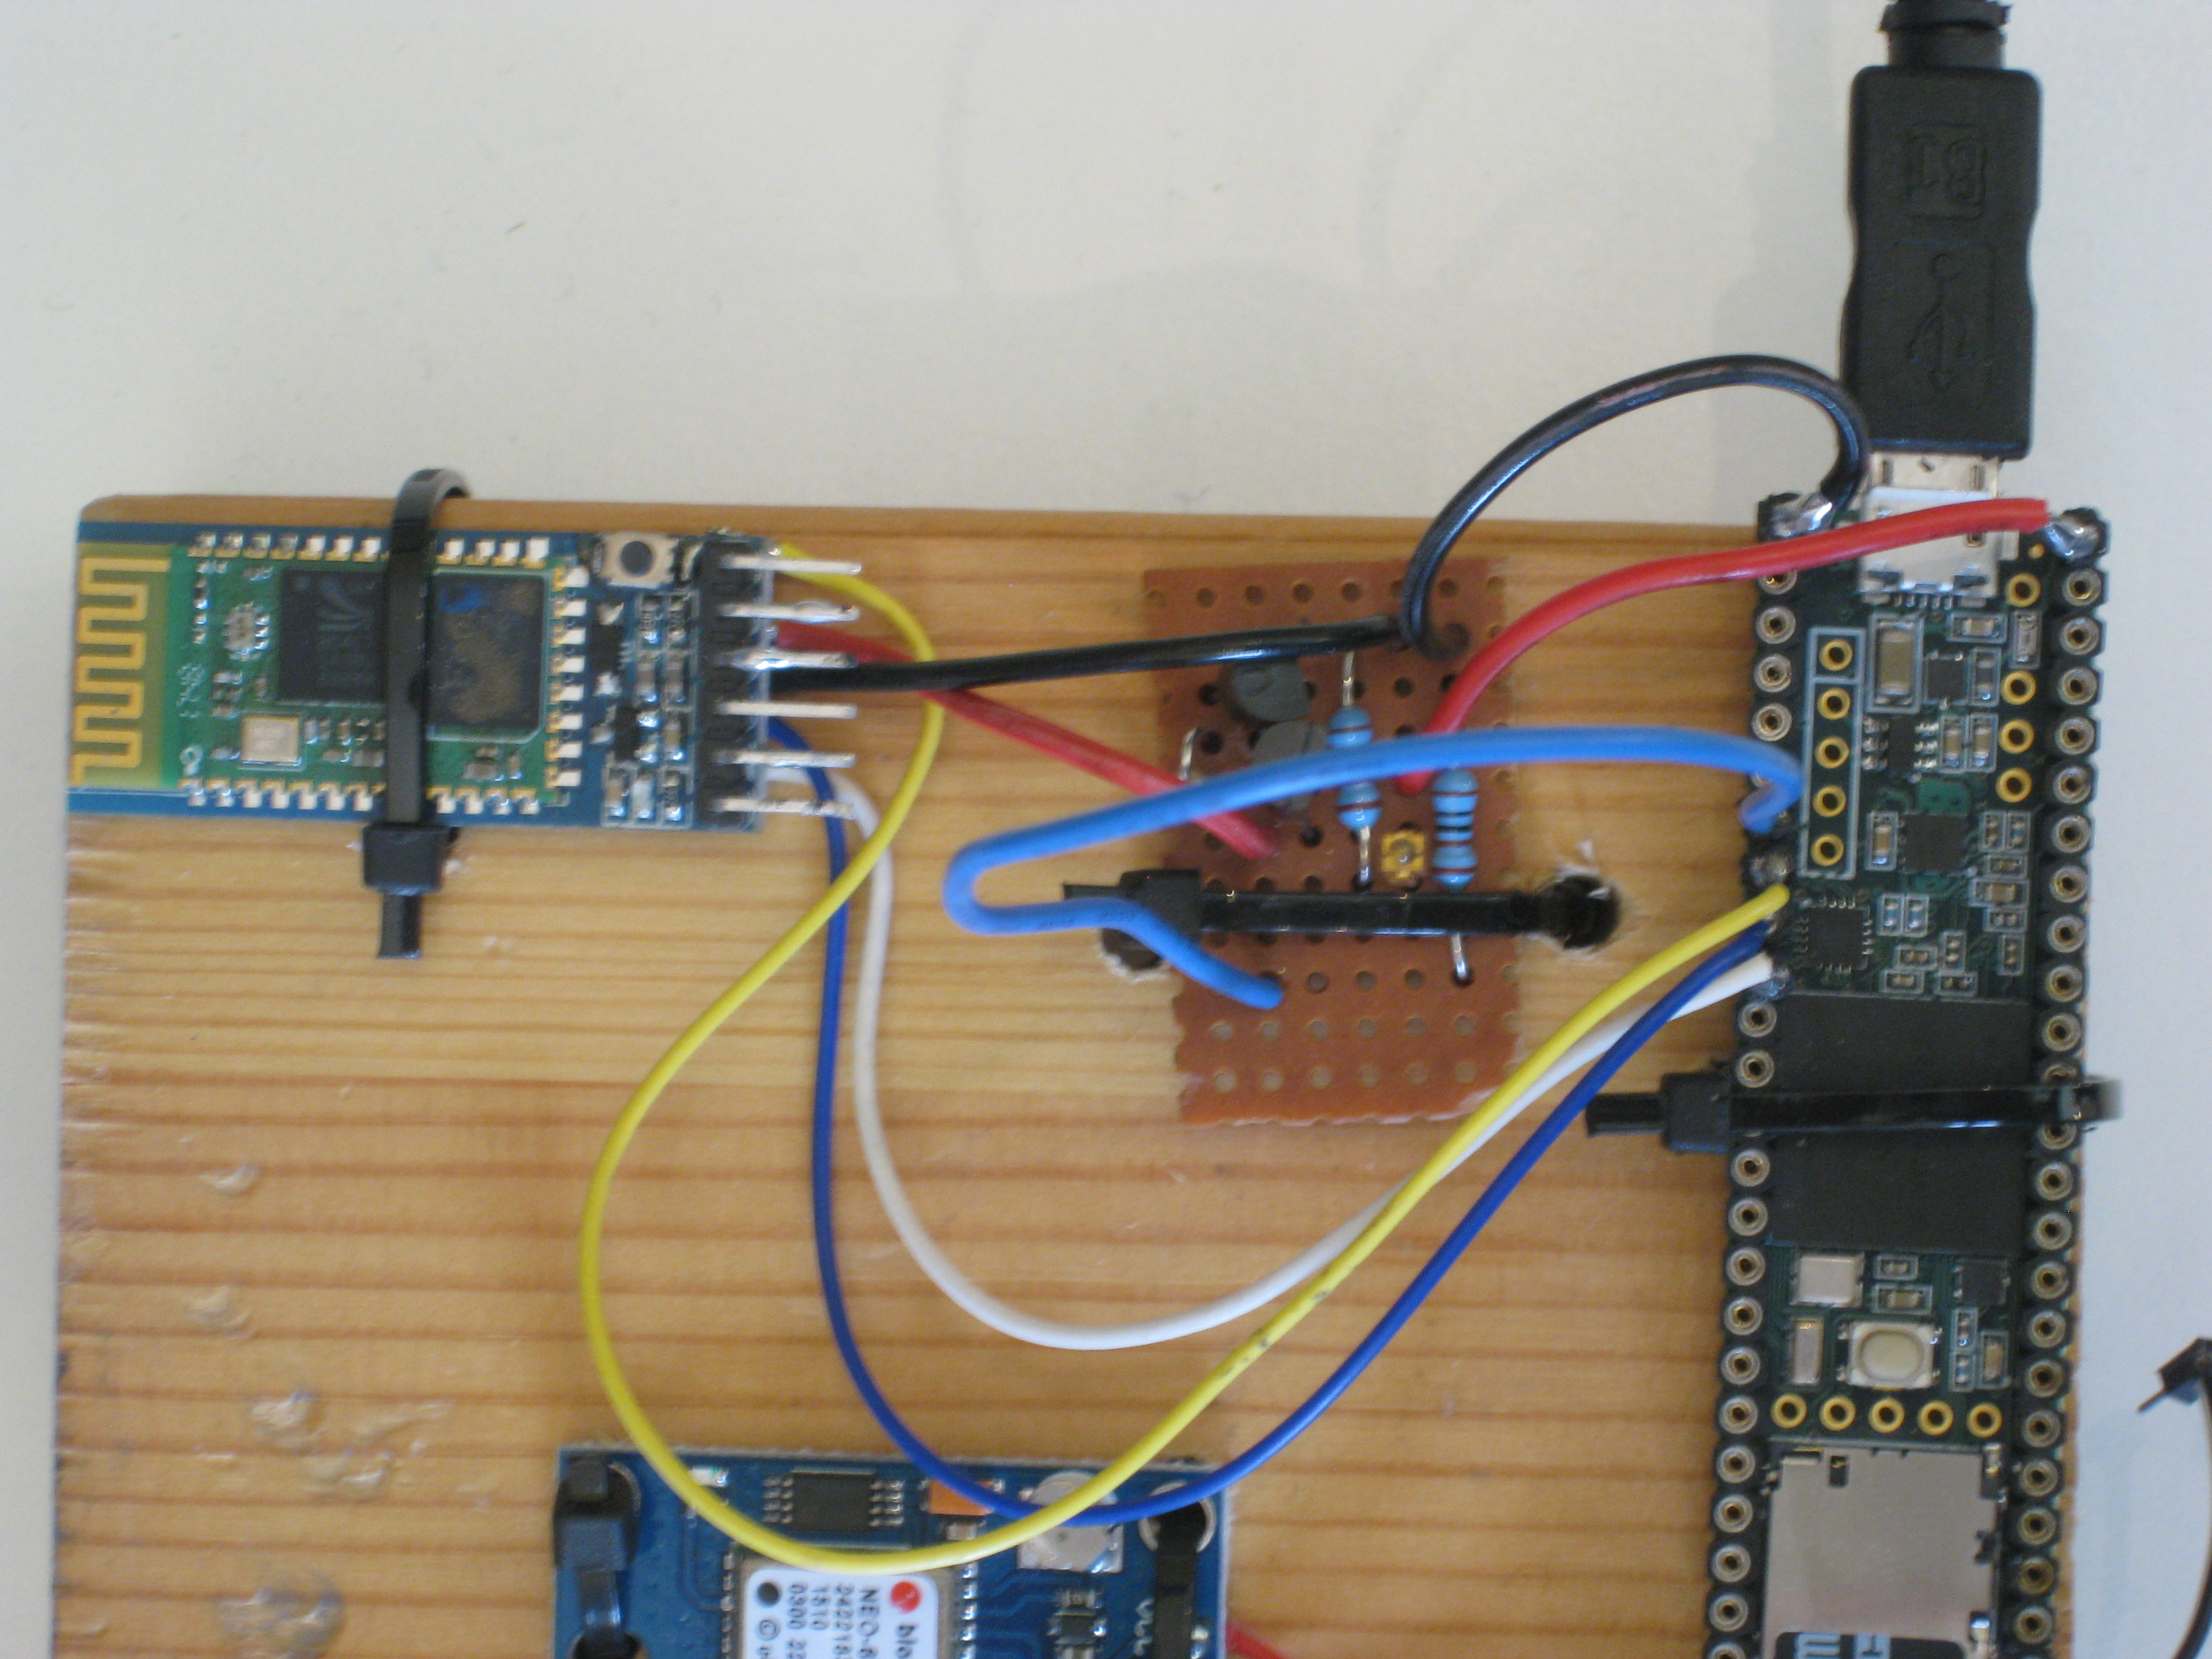
\includegraphics[width=.95\linewidth]{BT.JPG}\caption{Bluetooth-Modul und Schaltung zur Spannungsversorgung}
\end{figure}

Zunächst wir das Modul im AT-Modus konfiguriert und anschließend abgeschaltet, indem es von der Stromversorgung getrennt wird. Diese Trennung führen wir durch einen logischen Pegel (hellblau) herbei, den wir an einen der Transistoren zwischen der Stromquelle (dem 5V-Pin des Teensy) und dem VCC-Pin des Moduls eingebaut haben. Zu Debug-Zwecken ist afu der Platine eine LED (zwischen den beiden Wiederst"anden) verbaut, die leuchtet, solange das Modul mit Strom versorgt ist. Aufgrund der Hardwarelatenzen ben"otigen wir zum An- und Abschalten des Moduls jeweils circa 1,5~Sekunden, was die Zeit zur Erfassung aller Daten an einem GPS-Punkt deutlich verl"angert. Um mit der Datenerfassung zu beginnen, aktivieren wir das Modul im Inquire-Mode und lesen die Ankommenden Daten ein. Nach 10 Sekunden schalten wir das Modul wieder ab und lesen die restlichen Daten, welche eventuell im Puffer des Teensy liegen ein. Wir erhalten einen String, den wir an den Zeilenumbr"uchen trennen, um die einzelnen Datentupel zu isolieren. Anschlie"send filtern wir mithilfe regul"arer Audr"ucke die validen Tupel, um sie weiter zu verarbeiten. Dabei gehen wir ab diesem Punkt analog zum WLAN vor.\\
Durch die Latenzen und die relativ lange Erfassungzeit dauert eine Abfrage der Bluetooth-Ger"ate etwa 14,5 Sekunden und nimmt somit einen Gro"steil der gesamten Erfassungszeit ein. Diesen Kompromiss sind wir eingegangen, um die Erfassung der Bluetooth-Daten zu erm"oglichen.
\subsection{GSM-Modul SIM800L}
Das SIM800L-Modul hat uns gr"o"sere Schwierigkeiten bereitet, als alle anderen Module. Bis zuletzt war es uns nicht m"oglich es einzubinden. Eine Schwierigkeit bestand darin, dass verschiedene Bibliotheken f"ur das Modul existieren, welche sich bei bereits bei der Initialisierung unterscheiden. Auch gibt es widerspr"uchliche Aussagen dar"uber, ob die verwendete Simkarte pingesch"utzt sein darf oder nicht.\\
Das gr"o"ste Problem jedoch ist, dass das Modul, unabh"angig von der verwendeten Bibliothek auf keine Eingaben reagiert. Es soll, wie alle anderen Module, per UART auf AT-Befehle reagieren, erzeugte bei unseren Tests jedoch nie eine Antwort. 
F"ur verschiedene Szenarien haben wir Schaltungen eingebaut und getestet. Ohne anliegende Spannung am Reset-Pin, mit Reset beim Start auf high und anschlie"send low, und konstant high oder low war es uns nicht m"oglich vom Modul eine Antwort zu erhalten. Somit mussten wir schlie"slich die Einbindung des GSM-Moudls aufgeben.
\section{Fazit}
*** Mit etwas mehr Geld wären funktionierende Komponenten drin gewesen, aber so mit den seltsamen Eigenschaften klar zu kommen war eine interessante Erfahrung -> wenn man sich die teile später nicht immer aussuchen darf. ***
\nocite{*}
%\printbibliography[heading=head]%\addcontentsline{toc}{chapter}{Literatur}
\end{document}
